\documentclass[class=report, crop=false, 12pt,a4paper, tikz, border=4mm]{standalone}
\usepackage{enumitem}
\usepackage{float}
\usepackage{amsmath}
\usepackage{amssymb}
\usepackage[normalem]{ulem}
\usepackage{graphicx}
\usepackage{siunitx}
\usepackage{commath}
\usepackage{tikz}
\usetikzlibrary{positioning, fit, calc}   
\tikzset{block/.style={draw, thick, text width=3cm ,minimum height=1.3cm, align=center},   
line/.style={-latex}     
}
\begin{document}
\section{Impulse functions/responses}
\subsection{Impulse response of a system: Dirac delta function}
A useful tool in analysing the transient response of a system is the impulse signal, a unit (amplitude = 1) pulse infinitesimally small, with area = 1. Formally this is known as the \textbf{Dirac delta function (impulse function)}.
\begin{figure}[H]
  \centering
  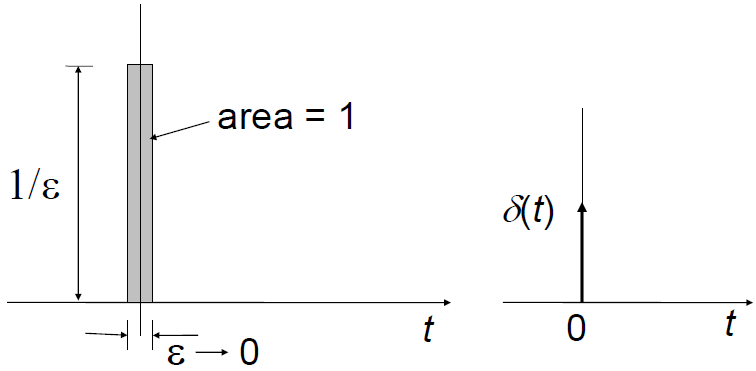
\includegraphics[width = 0.8\textwidth]{../img/diagram23.png}
\end{figure}
The Dirac delta function is a non-physical, singularity function with the follow definition:
\begin{equation}
  \delta (t) = \begin{cases}
    0 \textrm{ for } t \neq 0\\
    \textrm{undefined for } t = 0 
  \end{cases}
\end{equation}
but with the requirement that
\begin{equation}
  \int_{-\infty}^{\infty} \delta (t) \,\mathrm{d}t =1
\end{equation}
so taking the Laplace transform of this is also just 1
\begin{equation}
  \mathcal{L} (\delta (t)) = \int_{0^-}^{\infty} \delta (t) e^{-st} \,\mathrm{d}t = 1 
\end{equation}
Thus, the impulse response of the system is equal to the transfer function and from this it can be shown that \textbf{any} arbitrary signal can be described as a summation of impulse responses.
\subsection{Impulse response on a first order system}
Take a first order response for example, the transfer function and thus the impulse response looks like this:
\begin{figure}[H]
  \centering
  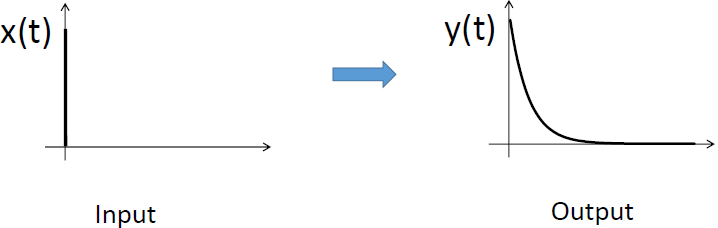
\includegraphics[width = 0.8\textwidth]{../img/diagram24.png}
\end{figure}
Due to our LTI assumptions:
\begin{itemize}
  \item Scaling the input scales the output
  \item Superposition of inputs equals superposition of outputs
  \item Time invariance
\end{itemize}
\subsection{Impulse response of a system}
\begin{figure}[H]
  \centering
  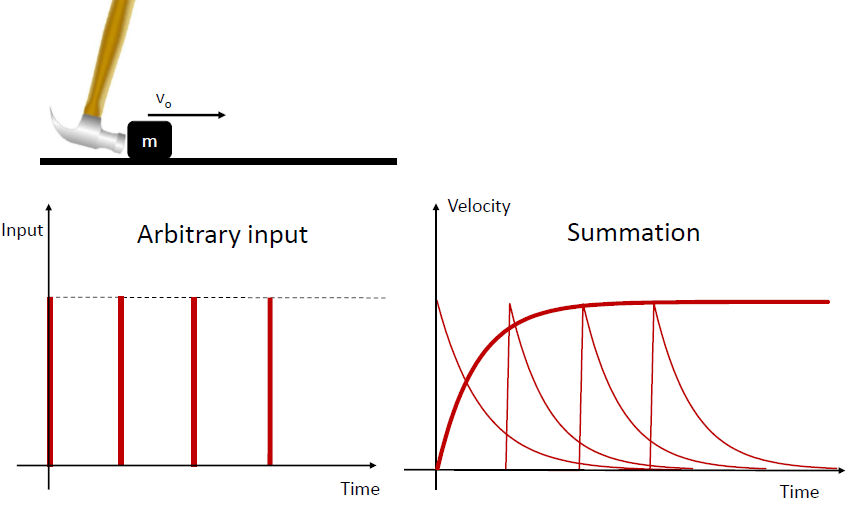
\includegraphics[width = 0.8\textwidth]{../img/diagram25.png}
\end{figure}
\subsubsection{Time vs Frequency Domain}
\begin{figure}[H]
  \centering
  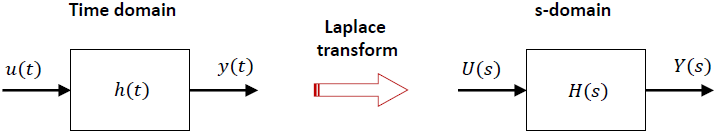
\includegraphics[width = 0.8\textwidth]{../img/diagram26.png}
\end{figure}
\begin{itemize}
  \item $u$ is the impulse function to the system
  \item $h$ is called the impulse response of the system
  \item $H$ is called the transfer function (TF) of the system
\end{itemize}
\begin{equation}
  y(t) = \int_{0}^{\infty} h(\tau) u (t-\tau) \,\mathrm{d}\tau = \int_{0}^{\infty} h(\tau - t)u(\tau) \,\mathrm{d}\tau  
\end{equation}
with $0\leq \tau \leq t$
\begin{equation}
  y(t) = h(t) \cdot u(t)
\end{equation}
This is called convolution.
\begin{equation}
  Y(s) = H(s) \cdot U(s)
\end{equation}
This is called multiplication.
\subsubsection{Convolution example}
Essentially, the steps for convolving two signals are to first reflect the signal $g$, then offset the reflected signal. Then calculate the area under the graph for every offset, by sliding $-g$. The convolution at each time point is equal to the area under the intersection of functions. For two pulses, the result is a triangle wave:
\begin{figure}[H]
  \centering
  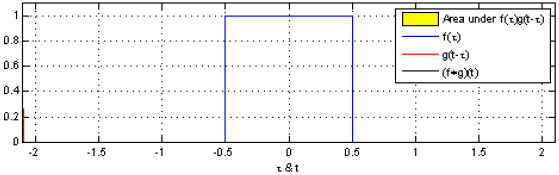
\includegraphics[width = 0.8\textwidth]{../img/diagram27.png}
\end{figure}
However, the calculations to obtain this result in the time domain are complicated, but are only multiplication in the Laplace domain.
\subsubsection{Getting the Time Response}
The procedure to describe the time response for LTI systems is thus:
\begin{itemize}
  \item Express the input, $u(t)$, in Laplace notation, $U(s)$
  \item Use this to find output $Y(s)$, usually by multiplying $U(s)$ by the transfer function $Y(s) = U(s)G(s)$
  \item Use inverse Laplace transforms (from tables) to express $Y(s)$ as a function of time, $y(t)$
\end{itemize}
\section{Input functions: Impulse - Step - Ramp}
Now we will consider some standard inputs and look at the response of first and second order systems:
\begin{itemize}
  \item Impulse
  \begin{itemize}
    \item The Laplace transform is 1, so the response to an impulse is by the definition the transfer function
  \end{itemize}
  \item Step
  \item Ramp
\end{itemize}
There are many others, particularly sinusoidal inputs or other discontinuous inputs, which are important in control loops, but we will focus on the two classic examples.
\subsection{Step input}
A step input is a discontinuous function, which is zero for all negative values of $t$ and 1 for all positive values.
\begin{figure}[H]
  \centering
  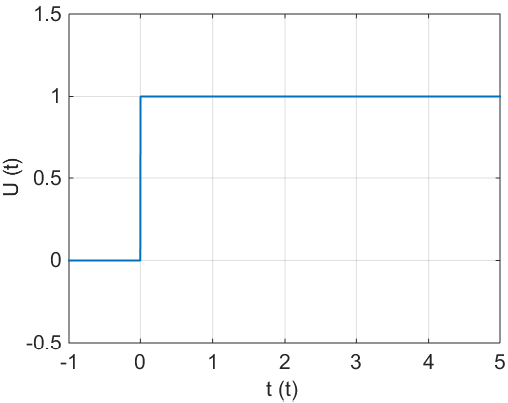
\includegraphics[width = 0.8\textwidth]{../img/diagram28.png}
\end{figure}
\subsubsection{Laplace transform}
\begin{gather}
  x(t) = U(t)\\
  \mathcal{L} \left\{ U(t) \right\} = \int_{0^-}^{\infty} e^{-st} \,\mathrm{d}t = \left[-\frac{1}{s} e^{-st}\right]_{0^-}^{\infty} \rightarrow \frac{1}{s}\\    
\end{gather}
Or for a gain of A
\begin{gather}
  x(t) = AU(t) \\
  \mathcal{L} \left\{ AU(t) \right\} = \frac{A}{s} 
\end{gather}
\subsubsection{Applications}
The step response is extremely useful in control theory for describing the behaviour of the system. In part because it incorporates the "transient" behaviour - from the sudden change from zero to one, as well as the "steady state" behaviour as the system settles down to a single value. IT also replicates many real world control applications such as:
\begin{itemize}
  \item Position control - move to a $X=10\si{\milli\meter}$ position and stay
  \item Speed control - go to 33 RPM
  \item Temperature - heat element on 3D printer to 230 \si{\celsius}
\end{itemize}
Also, unlike the Dirac impulse - it is physically realisable.
\subsection{Ramp input}
A ramp input has a value of $t$ for all $t$ values above zero and zero elsewhere, often is scaled by a gain A.
\begin{figure}[H]
  \centering
  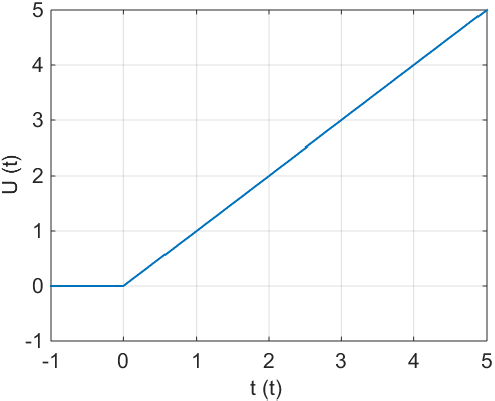
\includegraphics[width = 0.8\textwidth]{../img/diagram29.png}
\end{figure}
\subsubsection{Laplace transform}
\begin{gather}
  x(t) = at\\
  \mathcal{L} \left\{ at \right\} \int_{0^-}^{\infty} ate^{-st} \,\mathrm{d}t = -a \left[ \frac{t}{s}e^{-st} \right]_{0}^{\infty} + a\int_{0}^{\infty} \frac{1}{s} e^{-st} \,\mathrm{d}t\\
  = a \left[ -\frac{1}{s^2}e^{-st} \right] \rightarrow \frac{a}{s^2}   
\end{gather}
\subsubsection{Applications}
Ramp inputs are useful in understanding the steady state behaviour of a system i.e. when $t$ goes to infinity. Practical examples of control applications using ramp inputs are
\begin{itemize}
  \item Servo motors - shaft \textbf{position} rather than speed
  \item Ovens for PCB manufacturing etc. - strict linear \textbf{profile} of temperature required as opposed to "get to this temperature quickly"
  \item CNC milling machine, move in $X$ direction and constant rate
\end{itemize}
\subsection{Summary of Input Functions}
\begin{gather}
  \textrm{Impulse } F(s) = A\\
  \textrm{Step } F(s) = \frac{A}{s}\\
  \textrm{Ramp } F(s) = \frac{A}{s^2}
\end{gather}
For a \textbf{unit} response, $A=1$. We can apply these inputs to the LTI system by multiplying the transfer function by the input, both in terms of $s$.
\begin{figure}[H]
  \centering
  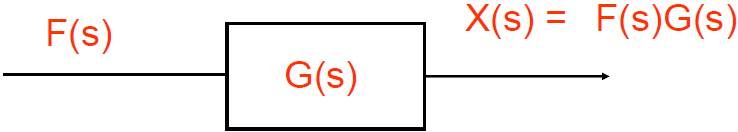
\includegraphics[width = 0.8\textwidth]{../img/diagram30.png}
\end{figure}
\section{First Order System Step Response}
Electromagnets are used in motors both rotary and linear, as well as in power transfer and also magnetic levitation in trains. First obtain the transfer function.
\begin{equation}
  \frac{I(s)}{V(s)}
\end{equation}
Balancing voltage gives:
\begin{equation}
  v(t) = v_R(t) + v_I(t)
\end{equation}
where
\begin{gather}
  v_R(t) = i (t) R\\
  v_I (t) = L\frac{\dif i(t)}{\dif t}
\end{gather}
Substitution gives:
\begin{equation}
  v(t) = Ri(t) + L\frac{\dif i(t)}{\dif t}
\end{equation}
In the Laplace domain
\begin{gather}
  V(s) = RI(s) + LsI(s)\\
  \frac{I(s)}{V(s)} = \frac{1}{(Ls + R)}
\end{gather}
For a \textbf{step} input of 1 \si{\volt} (unit step)
\begin{gather}
  V(s) = \frac{1}{s}\\
  I(s) = V(s) \frac{1}{(Ls + R)}\\
  =  \frac{1}{s(Ls + R)}
\end{gather}
Sadly there is no direct equivalent in the tables for this transform. The first takes is to split the expression up using partial fractions, into expressions that are give in the tables.
\begin{gather}
  I(s) = \frac{1}{s(Ls + R)} = \frac{\frac{1}{L}}{s(s+\frac{R}{L})} \textrm{ (remove coeff for s)}\\
  = \frac{k_1}{s} + \frac{k_2}{(s + \frac{R}{L})} \textrm{ partial fraction expansion}
\end{gather}
where
\begin{equation}
  k_1 (s + \frac{R}{L}) + k_2 s = \frac{1}{L}\\
\end{equation}
Looking at $s=0$
\begin{equation}
  k_1 \frac{R}{L} = \frac{1}{L} \rightarrow k_1 = \frac{1}{R}\\
\end{equation} 
Looking at $s= -\frac{R}{L}$
\begin{equation}
  -k_2 \frac{R}{L} = \frac{1}{L} \rightarrow k_2 = -\frac{1}{R}
\end{equation}
Which yields
\begin{equation}
  I(s) = \frac{1}{R} \left[ \frac{1}{s} - \frac{1}{(s+\frac{R}{L})} \right]
\end{equation}
Looking at the Laplace tables, we can now use entries for $\frac{1}{s}$ and $\frac{1}{(s + a)}$, considering $t > 0 \therefore u(t) = 1$.
\begin{equation}
  I(t) = \frac{1}{R} \left[ 1 - e^{-\frac{R}{L}t}\right]
\end{equation}
Which has the familiar form of a first order exponential rise, with a steady state gain of $\frac{1}{R}$. Time constant $\tau = \frac{L}{R}$. For now assume that $L$ and $R = 1$, so gain and time constant are 1.
\begin{figure}[H]
  \centering
  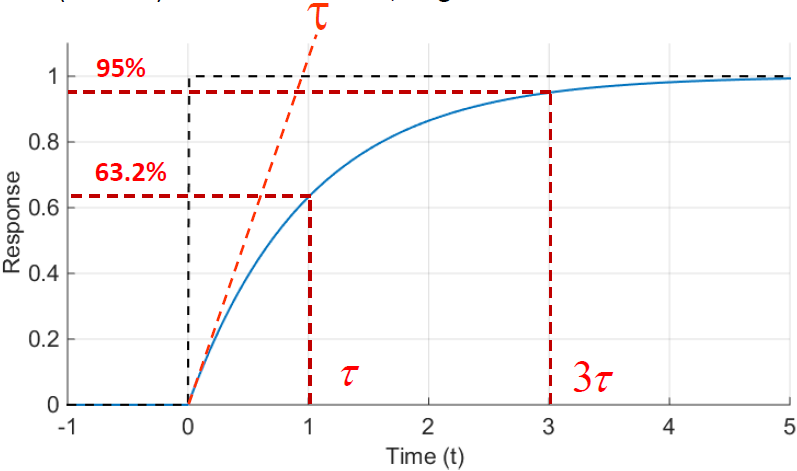
\includegraphics[width = 0.8\textwidth]{../img/diagram31.png}
\end{figure}
Thus for a known time constant, it is possible to calculate the response at any point after the step. A common parameter of a first order system is the \textbf{settling time} which is the time taken to reach 95\% of the desired value, or $3\tau$. The inverse process is also used in system identification, because the response is so simple - we can measure the step response and calculate the time constant of the system. If we do convolution in the time domain you get the same too.
\begin{figure}[H]
  \centering
  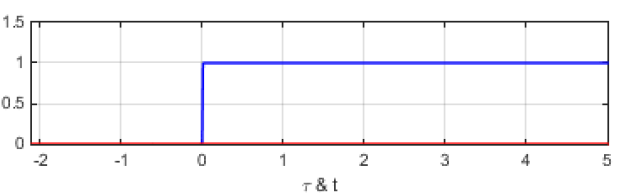
\includegraphics[width = 0.8\textwidth]{../img/diagram32.png}
  \caption{Area under $f(\tau)g(1-\tau)$, blue line $f(\tau)$, red line $g(t-\tau)$, black line $(f+g)t$.}
\end{figure}
These "step responses" can be repeated for different values of $V$ and for different starting values of $I(t)$. The response will always be behind the input for all time constant $>0$, and thus these systems are referred to as \textbf{first order lags}.
\begin{figure}[H]
  \centering
  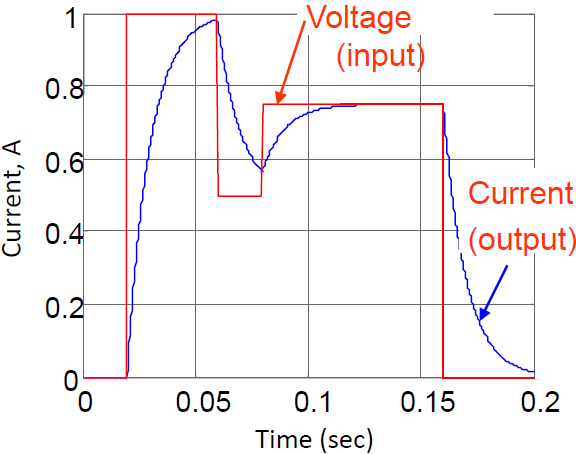
\includegraphics[width = 0.6\textwidth]{../img/diagram33.png}
\end{figure}
\section{First Order System Ramp Response}
For a \textbf{ramp} input of gain 1 (unit ramp)
\begin{gather}
  \frac{I(s)}{V(s)} = \frac{1}{(Ls+R)}\\
  V(s) = \frac{1}{s^2}\\
  I(s) = \frac{1}{s^2(Ls+R)} = \frac{\frac{1}{L}}{s^2(s+\frac{R}{L})}
\end{gather}
Again, this is not in the Laplace tables, so rearrange use partial fractions, giving us the general solution:
\begin{equation}
  I(t) = t - \tau \left(1 - e^{-\frac{t}{\tau}}\right)
\end{equation}
\begin{figure}[H]
  \centering
  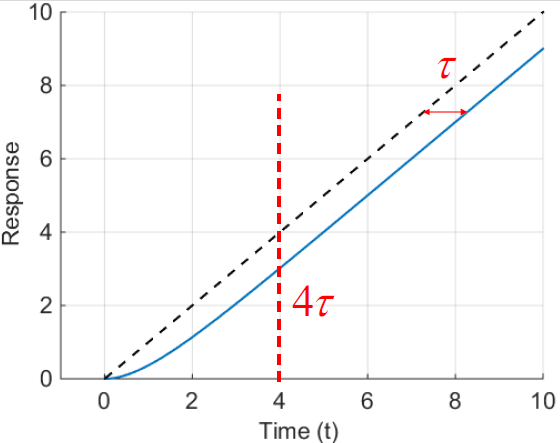
\includegraphics[width = 0.6\textwidth]{../img/diagram34.png}
\end{figure}
After 4 time constants, we can say that the system is in the \textbf{steady state} where the difference between the input and output is no longer changing. The steady state lag is then equal to $\tau$
\section{Understanding Poles and Zeros}
As defined, the transfer function is a rational function in the complex variable $s = \sigma + jw$, that is
\begin{equation}
  G(s)=\frac{b_ms^m + b_{m-1}s^{m-1} + ... + b_1s + b_0}{a_ns^n + a_{n-1}s^{n-1}+...+a_1s + a_0}
\end{equation}
It is often convenient to factor the polynomials in the numerator and denominator, and to write the transfer function terms of those factors:
\begin{equation}
  G(s) = \frac{N(s)}{D(s)} = K \frac{(s-z_1)(s-z_2)...(s-z_{m-1})(s-z_m)}{(s-p_1)(s-p_2)...(s-p_{n-1})(s-p_n)}
\end{equation}
Where the numerator and denominator polynomials, $N(s)$ and $D(s)$, have real coefficients defined by the system's differential equation and $K = \frac{b_m}{a_n}$. Poles and zeros are found by
\begin{equation}
  N(s) = 0 \textrm{ and } D(s) = 0
\end{equation}
All of the coefficients of polynomials $N(s)$ and $D(s)$ are real, therefore  the poles and zeros must be either purely real, or appear in complex conjugate pairs.
\begin{quotation}
  The poles and zeros are properties of the transfer function and therefore of the differential equation describing the input-output system dynamics. Together with the gain constant, they completely characterize the differential equation, and provide a complete description of the system.
\end{quotation}
\subsection{Example}
A linear system is described by the differential equation:
\begin{gather}
  \frac{\dif^2y}{\dif t^2} + 2\frac{\dif y}{\dif t} + 5y = 3\frac{\dif u}{\dif t} + 12u\\
  \mathcal{L} \left\{ \frac{\dif^2y}{\dif t^2} + 2\frac{\dif y}{\dif t} + 5y \right\} = s^2 Y(s) + 2sY(s) + 5Y(s)\\
  \mathcal{L} \left\{ 3\frac{\dif u}{\dif t} + 12u \right\} = 3sU(s) + 12U(s)\\
  N(s) = 3s + 12 = 0 \rightarrow z_1 = -4\\
  D(s) = s^2 + 2s + 5 \rightarrow p_{1/2} = \frac{-2 \pm \sqrt{2^2 - 4\times 5}}{2} = -1 \pm j2\\
  G(s) = \frac{N(s)}{D(s)} = 3 \frac{(s-(-4))}{(s-(-1+j2))(s-(-1-j2))} 
\end{gather}
\begin{figure}[H]
  \centering
  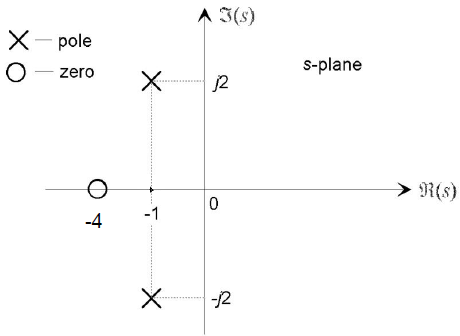
\includegraphics[width = 0.6\textwidth]{../img/diagram35.png}
\end{figure}
\subsection{s-Plane}
We can see how the time domain representation changes as we move around the s-plane. The imaginary axis corresponds to the sinusoidal component, and the real axis corresponds to the exponential.
\begin{figure}[H]
  \centering
  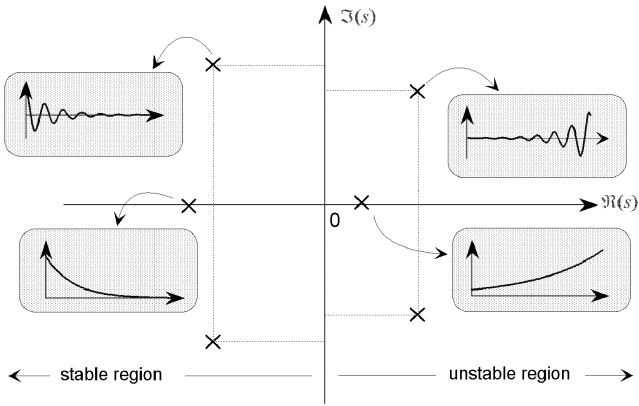
\includegraphics[width = 0.7\textwidth]{../img/diagram36.png}
\end{figure}
\section{Open Loop Motor Speed Control}
\begin{figure}[H]
  \centering
  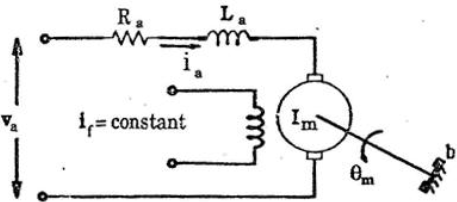
\includegraphics[width = 0.7\textwidth]{../img/diagram37.png}
\end{figure}
For a DC motor connected to an inertial load, there is a combination of electrical and mechanical system equations determining the transfer function for angular position with respect to voltage.
\begin{equation}
  \frac{\Theta_m (s)}{v_a(s)}
\end{equation}
First consider the voltage balance:
\begin{equation}
  v_a = R_a i_a + L_a \frac{\dif i_a}{\dif t} + e_m
\end{equation}
Where $e_m$ is the back e.m.f of the motor. We can also write the above in Laplace:
\begin{equation}
  V_a(s) = R_a I_a (s) + L_a s I_a (s) + E_m (s)
\end{equation}
Next consider the torque balance in motor:
\begin{equation}
  T(t) = I_m \frac{\dif^2 \theta_m}{\dif t^2} + b \frac{\dif \theta_m}{\dif t}
\end{equation}
Which gives the following in Laplace:
\begin{equation}
  T(s) = I_m s^2 \Theta_m + bs\Theta_m (s)
\end{equation}
The electrical and mechanical sides are connected by motor constant which describe the characteristics of the motor (and given by manufacturer).
\begin{gather}
  e_m = K_e \frac{\dif \theta_m}{\dif t} \\ 
  T = K_t i_a
\end{gather}
Or in the Laplace domain:
\begin{gather}
  E_m (s) = K_e s \Theta_m (s)\\
  T(s) = K_t I_a (s)
\end{gather}
Combining this with our previous equations:
\begin{gather}
  V_a (s) = R_a I_a (s)+L_a s I_a (s) + E_m (s)\\
  T(s) = I_m s^2 \Theta_m (s) + bs\Theta_m (s)
\end{gather}
We arrive at the equation of voltage with respect to angular position:
\begin{equation}
  V_a (s) = \frac{R_a b}{K_t} \left[ s(\tau_a s +1)(\tau_m s +1)\right] \Theta_m (s) + K_e s\Theta_m (s)
\end{equation}
"Armature" time constant related to electrical side:
\begin{equation}
  \tau_a = \frac{L_a}{R_a}
\end{equation}
Motor time constant related to mechanical side:
\begin{equation}
  \tau_m = \frac{I_m}{b}
\end{equation}
The transfer function the becomes:
\begin{equation}
  \frac{\Theta_m(s)}{V_a(s)} = \frac{\frac{K_t}{R_a b}}{s\left[ \tau_m \tau_a s^2 + (\tau_m + \tau_a)s + \left( \frac{K_e K_t}{R_a b} + 1 \right)  \right]}
\end{equation}
Which looks very complicated, but we can make some simplifying assumptions, which quickly make things simple again. The electrical time constant is normally very small when compared to the mechanical one, as manufacturers try to keep the resistance and inductance low, so we can neglect $\tau_a$. The result, then simplifies to the following equation:
\begin{gather}
  \frac{\Theta_m(s)}{V_a(s)} = \frac{K}{s(\tau s + 1)}\\
  K = \frac{K_a K_t}{(bR_a + K_t K_b)}
\end{gather}
Where $K$ is the remaining leftover constants. This looks \textbf{much} simpler now, but we can take a step further, rather than consider the output position, lets look at the transfer function with respect to speed $\omega$
\begin{gather}
  \frac{\omega_m (s)}{V_a (s)} = \frac{\dif \left( \frac{\Theta_m (s)}{V_a (s)} \right)}{\dif t} = s \left( \frac{K}{s(\tau s +1)} \right)\\
  \frac{\omega_m (s)}{V_a (s)} = \frac{K}{(\tau s +1)}
\end{gather}
This is now just a first order system.
\end{document}